\documentclass[]{article}

\usepackage{easyReview}

\usepackage{hyperref}

\usepackage{geometry} % Required for adjusting page dimensions and margins

\geometry{
	paper=a4paper, % Paper size, change to letterpaper for US letter size
	top=2.5cm, % Top margin
	bottom=3cm, % Bottom margin
	left=2.5cm, % Left margin
	right=2.5cm, % Right margin
	headheight=14pt, % Header height
	footskip=1.5cm, % Space from the bottom margin to the baseline of the footer
	headsep=1.2cm, % Space from the top margin to the baseline of the header
	%showframe, % Uncomment to show how the type block is set on the page
}

\usepackage{subfig}


\title{A graph-based approach for modification site assignment in proteomics}

\author{Dafni Skiadopoulou$^{1,2}$ \and Harald Barsnes$^{2,3}$ \and Lukas Käll$^{4}$ \and Marc Vaudel$^{1,2,5}$}
\date{%
	$^1$Mohn Center for Diabetes Precision Medicine,
	Department of Clinical Science,
	University of Bergen, Bergen, Norway\\%
	$^2$Computational Biology Unit,
	Department of Informatics,
	University of Bergen, Bergen, Norway\\%
	$^3$Proteomics Unit, 
	Department of Biomedicine, 
	University of Bergen, Bergen, Norway\\%
	$^3$Science for Life Laboratory,
	School of Engineering Sciences in Chemistry, Biotechnology and Health,
	KTH Royal Institute of Technology, Stockholm, Sweden\\
	$^4$Department of Genetics and Bioinformatics, Health Data and Digitalization,
	Norwegian Institute of Public Health, Oslo, Norway\\
}


\begin{document}
	
\maketitle

\subsection*{Abstract} 

\textbf{Summary:} 
	Assigning protein post-translational modifications to acceptor sites requires the distribution of modifications in a way that maximizes localization scores while avoiding chemically impossible configurations. We provide an efficient graph-based approach to this problem implemented both as standalone implementation and integrated in the PeptideShaker software tool. \\
\textbf{Availability and Implementation:} 
	An open source implementation in Python is available at https://github.com/ProGenNo/peptides-modifications-matching under a GPL-3.0 license. An open source implementation in Java is available at github.com/compomics/compomics-utilities under an Apache-2.0 license. \\

\maketitle

\section{Introduction}

In mass spectrometry-based proteomics, mass spectra of fragmented peptides are matched against a database of protein sequences using a proteomic search engine, allowing the high throughput identification of peptide sequences together with their modification status \cite{Mass_spec_proteomics}. The localization of post-translational modifications (PTMs) on protein sequences is an important functional information \cite{Phosphoproteomics}. Furthermore, since amino acid substitutions can have the same mass difference as a modification, an incorrectly localized modification can be misinterpreted, yielding a false variant call \cite{SNPs_PTMs_same_mass}. To evaluate the localization of modifications on a peptide sequence, multiple localization scores were developed that estimate the likelihood for a given acceptor site to be occupied for every modification of every peptide to spectrum match (PSM) \cite{Localization_scoring, computational_phosphoproteomics}.

Once the localization scores have been computed, the modifications are assigned to the sites of most likely localization before further processing, e.g. error rate estimation using Percolator \cite{Percolator}. It is important to note that due to differences in scoring, and especially since search engines often only consider the most intense peaks in mass spectra, the peptide maximizing the modification localization scores is not necessarily the best scoring peptide in the search engine results. And since the search engines also often have limitations in terms of how many modification sites combinations they consider, the peptide maximizing localization scores might not even be in the list of peptide candidates returned by the search engine.

In order to find the peptide maximizing the modification localization scores, the modifications found by the search engine need to be assigned to the site with highest localization score without yielding a configuration that is not chemically possible: modifications have different types of acceptor sites, e.g. amino acids or termini, and cannot be stacked on the same acceptor site. While maximizing the scores is trivial with a couple of modifications, e.g. phosphorylation and oxidation, the problem becomes more complex when combining many modifications with possible conflicting sites, e.g. in the study of histones \cite{Histone_study}. Furthermore, since this needs to be conducted on millions PSMs per experiment, the site assignment needs to be fast.

Here, we propose a graph-based approach that models modifications and their acceptor sites, and returns a configuration that maximizes localization scores with controlled processing time. The modification assignment problem is reduced to the maximum weight maximum cardinality matching problem in bipartite graphs, by modelling modifications and acceptor sites as vertices, connected by edges whose weights are calculated based on the corresponding modification localization scores. We provide a standalone Python implementation as well as a Java implementation in the compomics-utilities library \cite{compomics} and demonstrate its usage in PeptideShaker \cite{PeptideShaker}.

\section{Methods}

\subsection{Model}

In this work the modification site localization problem is addressed by a graph approach. For each PSM, a weighted  bipartite graph ($G = \{V,E,w\}$) is used to model all possible combinations of modifications on the amino acid chain. In this graph we determine two kinds of vertices, the ones that represent the different modifications (i.e. $D = \{d_1, d_2, \dots, d_k\}$) and the ones that represent all their possible acceptor sites (i.e. $A = \{a_1, a_2, \dots, a_n\}$). The set of vertices $V$ is then formed by the union of the sets $A$ and $D$ (i.e. $V = A \cup D$). For example, a peptide carrying four acetylations and one dimethylation, and featuring eight acceptor sites on the amino acid chain where either modification can occur, then the model will have 13 vertices in total ($\|D\| = 5$, $\|A\| = 8$, hence $\|V\| = 13$). For each modification in $D$, an edge is formed between the its vertex and the vertex of each of its possible acceptor sites in $A$. A weight $w_{i,j}$ is assigned to each edge $e_{i,j}$ corresponding to the localization score of the modification $d_i$ to the acceptor site $a_j$.

Using this model we reduce the modification site assignment problem to the maximum weight maximum cardinality matching problem on the resulting bipartite graph. The solution of this problem will be a set of pairwise non-adjacent edges satisfying two conditions. The first one is that the matching will be of maximum cardinality, which in this modeling ensures that all the vertices that represent a modification will be matched. The second condition is that the weight of the matching is maximum, which means that it provides the combination of modifications and acceptor sites that gives the maximum localization score in total.


\subsection{Implementation}

We provide an open source Python-based implementation of our approach available under a GPL-3.0 license (github.com/ProGenNo/peptides-modifications-matching). For this we used the networkX \cite{networkX} library and its algorithm for the minimum weight full matching problem. This algorithm when applied on our model produces a matching $M$ with cardinality $\|M\| = min\{\|A\|, \|D\|\} = \|D\|$ which ensures that all the modifications will be matched to a site in the amino acid chain (because the model assumes that the graph is connected and there are at least as many possible acceptor sites as there are modifications, therefore $\|A\| \geq \|D\|$). However the algorithm produces a matching that minimizes the sum of weights of the corresponding edges. Therefore in order to be suitable for the modification assignment problem, the weights of the edges from the model described in this work were transformed accordingly so as the maximum localization score corresponded to the minimum edge weight. The script of the implementation receives as input a text file where a description of the available PSMs is included. It requires one line per PSM with the information of the spectrum and peptide IDs as well as the modifications with their possible acceptor sites and the corresponding localization scores. Exceptions are thrown for each PSM if there are fewer acceptor sites given than modifications, or if there is no possible full matching in the resulting graph or if the localization scores take negative values. Further information are available at the github repository. 

We also provide an open source Java-based implementation freely available as part of the compomics-utilities library \cite{compomics} under an Apache-2.0 license. It is located in the \textit{com.compomics.util.experiment.identification.modification.peptide\_mapping} package and makes use of the JGraphT package \cite{JGraphT}. This includes an implementation of the Kuhn-Munkres algorithm for the assignment problem, which requires as input a complete bipartite graph and produces a perfect matching with minimum weight. To make this algorithm suitable for the modification assignment problem the weights of the edges of the model proposed in this work were transformed as in the python implementation. Also, the graph model was made complete with the addition of dummy vertices and edges if needed, while ensuring that the perfect matching of minimum weight still corresponded to the best assignment of modifications to acceptor sites. For more information see the implementation in compomics-utilities, which is readily usable \textit{via} the PeptideShaker tool \cite{PeptideShaker}.

\comment{}{TODO Dafni: Write a more formal description of the transformation as a standalone paragraph.}
\comment{}{TODO Marc: Write wiki page in compomics-utilities}

\subsection{Histone example}

A dataset acquired on a synthetic histone peptide with different combinations of modifications was searched using MS-Amanda \cite{MS_Amanda} using SearchGUI \cite{SearchGUI}. The result file of MS-Amanda was processed using PeptideShaker where all modifications were scored using PhosphoRS \cite{PhosphoRS}.

\comment{}{TODO Marc: Check with Veit}

\subsection{Performance benchmark}

We generated sets of peptides of length 30 with multiple random sets of modifications. For each peptide, the number of distinct modifications was randomly generated between one and ten. For every modification, up to six modification sites were randomly selected, and the number of modified residues was randomly set between one and the number of modification sites. Finally, modification localization scores were given randomly for all modification sites and the matching of modification to site was conducted using the Java implementation. The code was run for different batches of peptides using different number of threads on a laptop computer, and the processing time was recorded. 

Subsequently, we generated peptides in a similar fashion, but fixed the number of distinct modifications, modification sites, and modified residues. We then benchmarked the processing time for all possible combinations using 1,000 peptides per thread and all threads available.

Each benchmark was replicated ten times. The code used to benchmark the application is available in the \textit{com.compomics.util.experiment.identification.modification.peptide\_mapping.performance} package of the compomics-utilities library.


\section{Results}

\subsection{Histone modification localization example}


 An example of a graph model for a modified peptide is presented in Fig. \ref{fig:histone_peptide}, where one site was reported by the search engine to carry a dimethylation and four were found to carry an acetylation. The maximum weight matching then assigned the modifications to the best scoring residues while avoiding to put the dimethylation on the same amino acid as an acetylation. As seen in this example, in case there are multiple combinations that give the same total sum of localization scores,  one of them will be chosen randomly. Note that our approach can be applied to peptides carrying any combination of modifications identified by proteomic search engines.
 
 \begin{figure}[!tpb]
 	\centerline{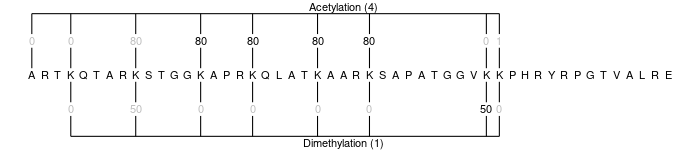
\includegraphics[width=0.6\textwidth]{figures/figure_histone.png}}
 	\caption{Graph representation of a peptide with four acetylations and one dimethylation with all their possible acceptor sites and the respective localization scores. The localization scores selected by the matching procedure are highlighted in black while the other ones are in gray. Note that in the actual graph representation of the model, the four acetylations are represented as four distinct vertices that are not represented on this figure for the sake of readability.}\label{fig:histone_peptide}
 \end{figure}
 

\subsection{Performance}

Benchmarking the performance of the matching algorithm demonstrated that around one million peptides could be processed per minute and per thread. Since the peptides are scored individually, they can be processed in parallel and as soon as approximately 1,000 peptides were available, the processing time increased linearly with the number of peptides and a minor increase in processing time was observed when using multiple threads, which we impute to Java having to manage many more objects (Figure \ref{fig:performance_threads}). For a given peptide, the modification matching time increased with the number of different modifications, the number of sites, and the number of modified residues (Figure \ref{fig:performance_size}). In all configurations, the modification site assignment took only few seconds for thousands of peptides, which is negligible compared to the search time, which can be of several hours, as was the case for the Histone example.

%\begin{figure}[!tpb]
%	\centerline{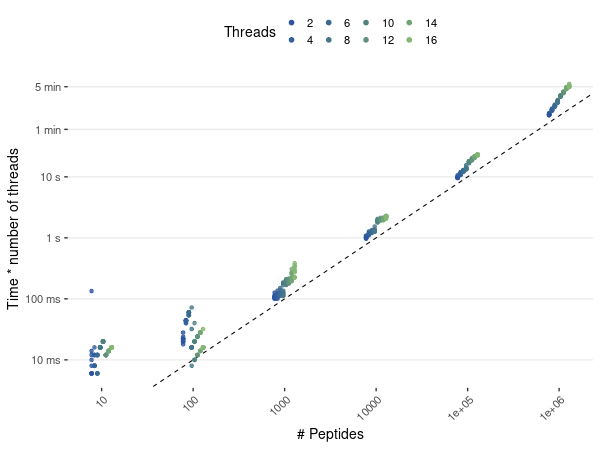
\includegraphics[width=0.6\textwidth]{figures/benchmark_23.02.02_threads.png}}
%	\caption{Processing time multiplied by the number of thread plotted against the number of peptides for benchmark runs of equal numbers of peptides. Note that log scales are used on both axes. Runs with different number of threads are jittered from left to right and plotted with different colors.}\label{fig:performance_threads}
%\end{figure}


%\begin{figure}[!tpb]
%\centerline{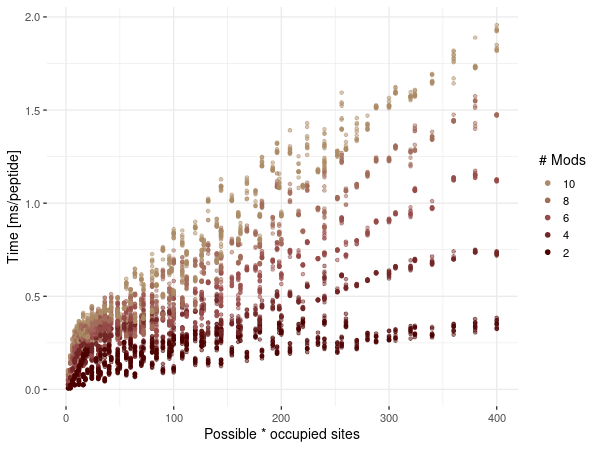
\includegraphics[width=0.6\textwidth]{figures/benchmark_23.02.02_size.png}}
%\caption{For different baches of 1,000 peptides per thread using 16 threads, processing time per peptide against number of sites multiplied by number of modified residues. Peptides with different number of distinct modifications are colored differently.}\label{fig:performance_size}
%\end{figure}

\begin{figure}[!ht]
	\subfloat[\label{fig:performance_threads}]{%
		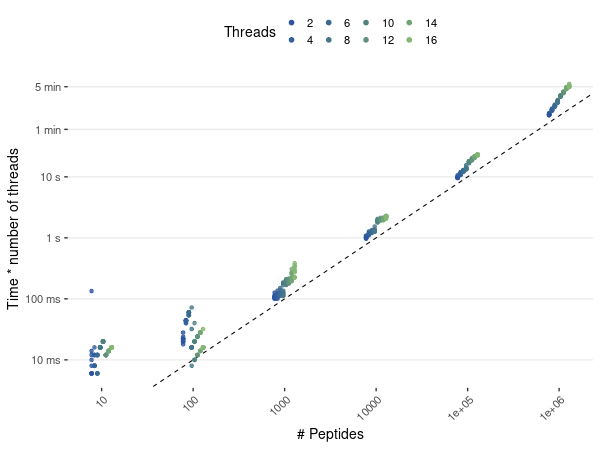
\includegraphics[width=0.49\textwidth]{figures/benchmark_23.02.02_threads.png}
	}
	\hfill
	\subfloat[\label{fig:performance_size}]{%
		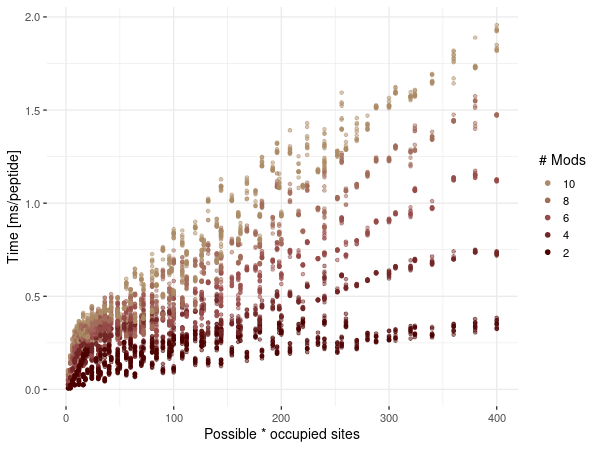
\includegraphics[width=0.49\textwidth]{figures/benchmark_23.02.02_size.png}
	}
	\caption{(a) Processing time multiplied by the number of thread plotted against the number of peptides for benchmark runs of equal numbers of peptides. Note that logarithmic scales are used on both axes. Runs with different number of threads are jittered from left to right and plotted with different colors. (b) For different baches of 1,000 peptides per thread using 16 threads, processing time per peptide against number of sites multiplied by number of modified residues. Peptides with different number of distinct modifications are colored differently.}
	\label{fig:performance_test}
\end{figure}


\section{Conclusion}

	This work addresses the problem of finding the optimal assignment of post translational modifications (PTMs) on the amino acid chain of peptides upon modification localization scoring in mass spectrometry-based proteomics. Given the possible modifications and all their acceptor sites together with the corresponding localization scores, the proposed graph approach finds the combination of modifications on the amino acid chain that maximizes the localization scores while avoiding impossible combinations. This approach thus enables the consolidation of modification localization scores for heavily modified peptides and thereby increases the performance of proteomic pipelines when multiple modifications are considered without substantially increasing processing time.


\section{Acknowledgements}

This work was supported by the Research Council of Norway (project \#301178 to MV) and the University of Bergen.

This research was funded, in whole or in part, by the Research Council of Norway 301178. A CC BY or equivalent license is applied to any Author Accepted Manuscript (AAM) version arising from this submission, in accordance with the grant’s open access conditions.


\bibliographystyle{ieeetr}

%\section*{\refname}
\bibliography{paper_PMMP}





\end{document}
